First of all, to be sure that the Taylor shift by 1 was done correctly, I needed some comparison, like using Maple, or other codes, in particular in C++. I used mainly the comparison of my CUDA code with the execution of the Horner's method in C++, which is the fastest compared to the Divide and Conquer method in C++ and the execution on Maple. \\

In the following graphics, MAPLE is not represented because the execution time increases by a factor of 4 each time we multiply by 2 the number of coefficients of the polynomial we want to be shifted by 1. Nevertheless, I show the execution time of the Maple script I used in the array of the execution times. \\

Here are the differents results obtained for different sizes of random polynomials. Let us recall that these polynomials are of degree $n = 2^e-1$ : \\

\begin{center}
\begin{tabular}{||c|c||c||r|r||r||}
   \hline
  \multicolumn{6}{||c||}{Execution time in seconds} \\
 \hline
  e  &    n    &    GPU     &  CPU : HOR  &   CPU : DNC  &  Maple 16   \\  \hline \hline
  3  &      8  &  0.001518  &   0.000128  &    0.000141  &     <0.001  \\
  4  &     16  &  0.001432  &   0.000186  &    0.000172  &     <0.001  \\
  5  &     32  &  0.001590  &   0.000167  &    0.000191  &     <0.001  \\
  6  &     64  &  0.001773  &   0.000192  &    0.000294  &      0.008  \\
  7  &    128  &  0.002016  &   0.000261  &    0.000628  &      0.024  \\
  8  &    256  &  0.003036  &   0.000593  &    0.002331  &      0.084  \\
  9  &    512  &  0.002624  &   0.001278  &    0.006304  &      0.320  \\
 10  &   1024  &  0.005756  &   0.005940  &    0.032073  &      1.400  \\
 11  &   2048  &  0.009317  &   0.015312  &    0.095027  &      5.640  \\
 12  &   4096  &  0.013475  &   0.076866  &    0.376543  &     24.478  \\
 13  &   8192  &  0.019674  &   0.324029  &    1.498890  &    104.438  \\
 14  &  16384  &  0.027229  &   1.282708  &    6.861433  &    437.848  \\
 15  &  32768  &  0.042561  &   5.110919  &   23.907799  &   1781.427  \\
 16  &  65536  &  0.064306  &  15.184347  &  114.988129  &   7407.063  \\
 17  & 131072  &  0.127214  &  80.625801  &  477.934692  &     >10000  \\
   \hline 
\end{tabular}
\end{center}

To compare more in details, take a look at the differents pictures we can have using gnuplot. Gnuplot scripts can be seen in the appendix. The execution times of MAPLE 16 don't appear as they increase too much compared to my other results. I show different graphics, considering $e$ in x-axis then $n$, as my results are for polynomials of size $2^e$. The results with $n$ in x-axis are more eloquent concerning the fact that the execution time becomes linears when $n$ increases by a factor of $2$.\\

\begin{center}
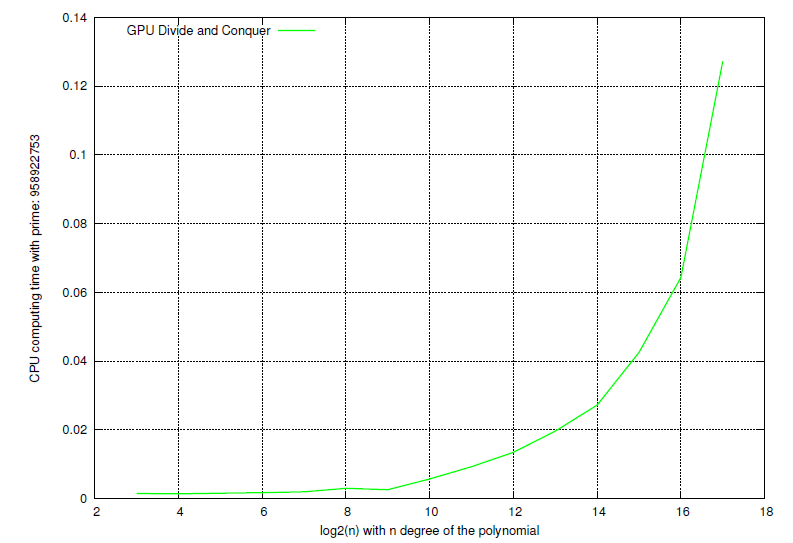
\includegraphics[scale=0.8]{eps/GPUtime_e.png}
\textbf{Execution time of the GPU in function of $e$}\\
\end{center}


The following graphic is more eloquent concerning the linear increasing of the execution time of the GPU depending on the power of $2$ the size of the polynomial is considered. Nevertheless, the execution is not really linear. Indeed, the cuda code contains also a part executed in serie, like when we read the polynomial in a file and also when we store the result in a file. \\

\begin{center}
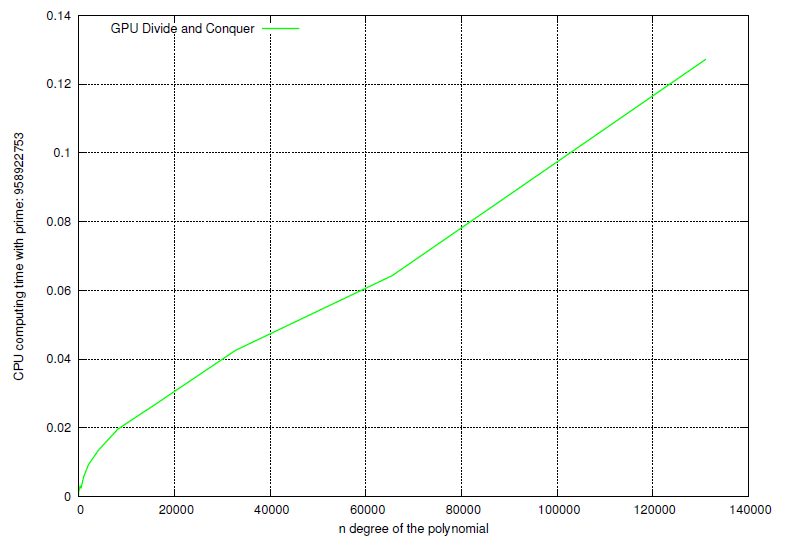
\includegraphics[scale=0.8]{eps/GPUtime_n.png}
\textbf{Execution time of the GPU in function of $n$}\\
\end{center}

Now let's take a look at the execution times for the Horner's method and for the Divide and Conquer method in serie, so with the CPU only. The two methods are not linear and increase by a factor of $4$ according to the previous array.\\

\begin{center}
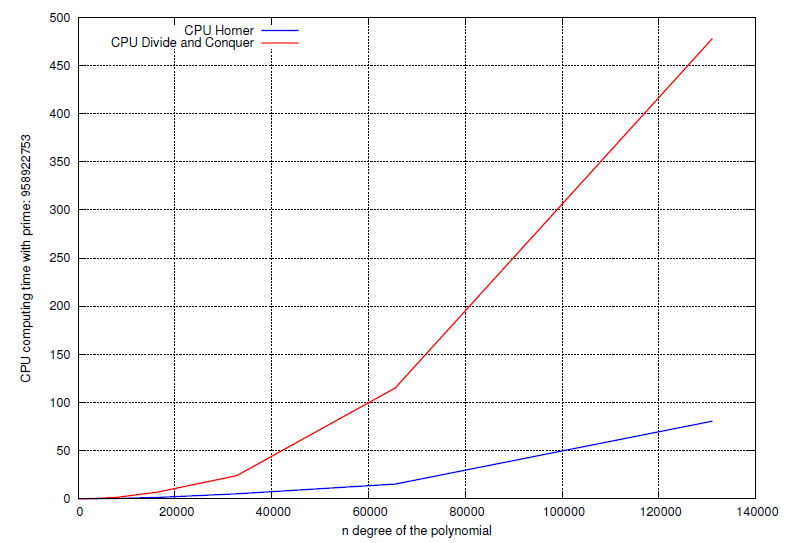
\includegraphics[scale=0.8]{eps/CPUtime_n.png}
\textbf{Execution time of the CPU in function of $n$}\\
\end{center}

We clearly see that the Horner's method in serie is more efficient than the Divide and Conquer method in serie. To see exactly what happen for small degrees and big degree for the three methods, namely the GPU DNC method, the CPU DNC method and the CPU Horner's method (when I say GPU I mean 'in parallel', and when I say CPU I mean 'in serie'). Let's consider the two following graphics.\\

\begin{center}
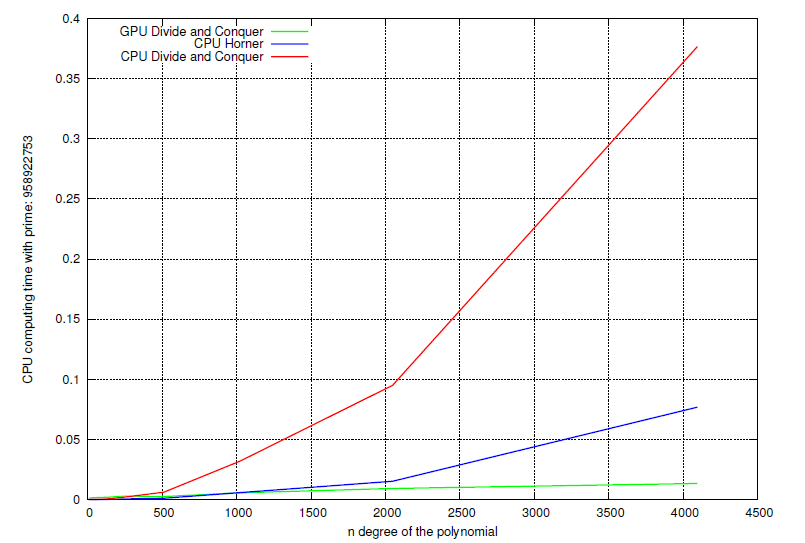
\includegraphics[scale=0.8]{eps/time_small_n.png}
\textbf{Execution times in function of $n$ for small degrees}\\
\end{center}

For small degrees, we see that the execution time of the GPU code is approximatively the same and worst than the execution times of the CPU execution times. The reasons are very simple, for small degrees, we need the same number of arrays in the CUDA code than for the big degrees, even though obviously they are not at the same size than for big degrees. Allocate memory for the GPU takes a lot of time at the scale of the execution times for small degrees, so finally there are a lot of communications just for 'small' computations. To conclude with this, for small degrees, it will be better to do the Taylor shift by 1 in serie. There is also the fact that we don't compute the same way the Taylor shift in the three methods, even though for the divide and conquer in serie, the only difference is the way we do the multiplication (and obviously the fact it is in serie).\\

Let's see the comparison for the next degrees :\\

\begin{center}
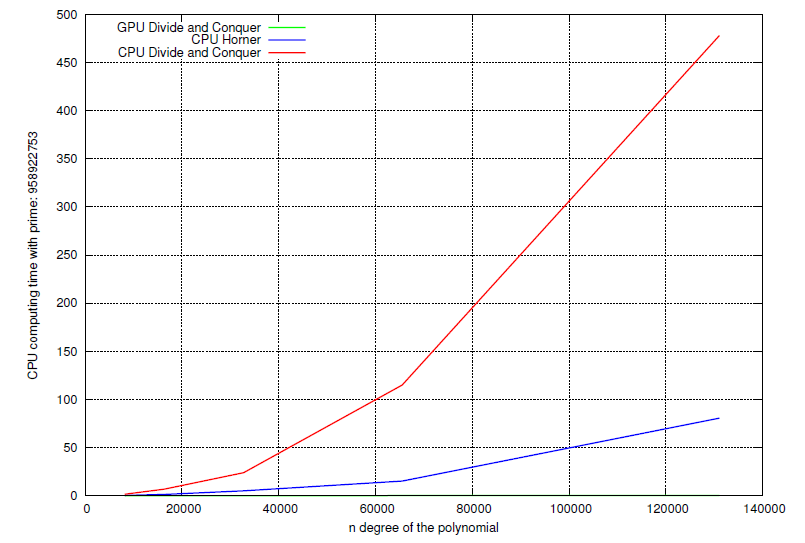
\includegraphics[scale=0.8]{eps/time_big_n.png}
\textbf{Execution times in function of $n$ for big degrees}\\
\end{center}

For big degrees, using the GPU gives best performances with a execution time of approximatively 0.1 second for a polynomial of size $2^{17}$. We see clearly a huge gap between the execution times of the different methods implemented, and remember that I didn't put the execution time using Maple also. We see that to parallelize the Taylor shift, is a real challenge, notably for MAPLE, which has finally the worst execution time for big degrees.
